\documentclass{grattan}\usepackage[]{graphicx}\usepackage[]{color}
%% maxwidth is the original width if it is less than linewidth
%% otherwise use linewidth (to make sure the graphics do not exceed the margin)
\makeatletter
\def\maxwidth{ %
  \ifdim\Gin@nat@width>\linewidth
    \linewidth
  \else
    \Gin@nat@width
  \fi
}
\makeatother

\definecolor{fgcolor}{rgb}{0.345, 0.345, 0.345}
\newcommand{\hlnum}[1]{\textcolor[rgb]{0.686,0.059,0.569}{#1}}%
\newcommand{\hlstr}[1]{\textcolor[rgb]{0.192,0.494,0.8}{#1}}%
\newcommand{\hlcom}[1]{\textcolor[rgb]{0.678,0.584,0.686}{\textit{#1}}}%
\newcommand{\hlopt}[1]{\textcolor[rgb]{0,0,0}{#1}}%
\newcommand{\hlstd}[1]{\textcolor[rgb]{0.345,0.345,0.345}{#1}}%
\newcommand{\hlkwa}[1]{\textcolor[rgb]{0.161,0.373,0.58}{\textbf{#1}}}%
\newcommand{\hlkwb}[1]{\textcolor[rgb]{0.69,0.353,0.396}{#1}}%
\newcommand{\hlkwc}[1]{\textcolor[rgb]{0.333,0.667,0.333}{#1}}%
\newcommand{\hlkwd}[1]{\textcolor[rgb]{0.737,0.353,0.396}{\textbf{#1}}}%

\usepackage{framed}
\makeatletter
\newenvironment{kframe}{%
 \def\at@end@of@kframe{}%
 \ifinner\ifhmode%
  \def\at@end@of@kframe{\end{minipage}}%
  \begin{minipage}{\columnwidth}%
 \fi\fi%
 \def\FrameCommand##1{\hskip\@totalleftmargin \hskip-\fboxsep
 \colorbox{shadecolor}{##1}\hskip-\fboxsep
     % There is no \\@totalrightmargin, so:
     \hskip-\linewidth \hskip-\@totalleftmargin \hskip\columnwidth}%
 \MakeFramed {\advance\hsize-\width
   \@totalleftmargin\z@ \linewidth\hsize
   \@setminipage}}%
 {\par\unskip\endMakeFramed%
 \at@end@of@kframe}
\makeatother

\definecolor{shadecolor}{rgb}{.97, .97, .97}
\definecolor{messagecolor}{rgb}{0, 0, 0}
\definecolor{warningcolor}{rgb}{1, 0, 1}
\definecolor{errorcolor}{rgb}{1, 0, 0}
\newenvironment{knitrout}{}{} % an empty environment to be redefined in TeX

\usepackage{alltt}

\title{Negative gearing distributions}
\author{Hugh Parsonage}

\addbibresource{bibliography.bib}

\newcommand\gao{Grattan analysis of}

\usetikzlibrary{shapes,arrows}
\tikzstyle{block} = [rectangle, draw, 
    text width=4em, text centered, rounded corners, minimum height=4em]
    
    \tikzstyle{line} = [draw, thick, -latex']

\newcommand{\EMPH}[1]{\textbf{#1}}
\newcommand{\highlight}[1]{\emph{#1}}
\IfFileExists{upquote.sty}{\usepackage{upquote}}{}
\begin{document}
\clearpage
%\chapter{Distribution of negative gearing}

\chapter{Other tax concessions for savings: capital gains tax discount and negative gearing}
Reducing the tax concessions for investments in housing and other assets are attractive reforms. 

This chapter examines two significant concessions in the taxation of savings: \highlight{tax discounts for capital gains} and \highlight{negative gearing}.\footnote{This report does not consider making owner-occupied housing liable for capital gains tax because of the significant negative social and econoimic consequences discussed in \textcite{Daley2013}.}  These allow investors to use debt financed investment, particularly property investment, to reduce and defer their personal income tax.

These tax concessions have reduced housing affordability. By increasing post-tax returns for property investors they increase investment in rental housing, pushing up prices to the disadvantage of young would-be home buyers. Like most tax concessions on investment, these concessions largely benefit the wealthy. 

Reducing these concessions would not have a large effect on savings rates or productive investment. Tax rates do not do much to affect the amount that wealthy people save - although they do affect the form of savings. Nor would abolishing these tax concessions lead to materially higher rents. History and economic theory suggest that changed tax concessions would alter property prices but not rent. 

Reducing these tax concessions would improve the budget bottom line. 

The 50 per cent CGT discount provides an annual tax discount to individuals and trusts worth \$7 billion each year.\footcite[p.~74]{Treasury2015a}  Reducing the discount to 30 per cent could raise around \$4 billion, depending on the extent of behavioural change. 

Negative gearing should also be limited. The tax deductibility of costs, including interest costs, prevents a tax bias against debt funding and more risky investments. But this does not mean that losses should be able to be written off against wage and salary income. Quarantining losses so they can only be written off against other investment income (operating profits and capital gains) could raise around \$4.2 billion a year in the short-term. This would decline to around \$1.5 billion over time as those losses are offset against investment income.  

An alternative option would align the tax rates for capital gains and losses.  For example, the capital gains discount could be reduced so that people paid tax on 70 per cent of their capital gains, but could claim only 70 per cent of any investment losses against wage and salary income. Treating capital gains and recurrent losses consistently would reduce the tax-driven incentive for borrowing to invest. It would contribute around \$4 billion a year to the bottom line. 

The current tax treatment of depreciation is also overly favourable to investors. Reform could raise an additional \$1 billion. 

The best way to transition to these new arrangements would be to phase them in over a number of years. Such a phase-in will help smooth reductions in asset prices and reduce the risk of over-shooting, and a broader economic slump. 

Alternatively, all assets bought before a specified date could be ``grandfathered'' so that the current tax concessions apply to them whenever they are sold, but not to newly purchased assets. Although grandfathering minimises the disappointment for existing investors, it encourages investors to ``hoard'' assets inefficiently. It also treats generations unfairly because it gives additional benefits to those with enough wealth to have bought already.

\section{Capital gains enjoy preferential tax treatment relative to income from working}
Capital gains are taxed as part of the income of individuals, companies and superannuation funds. In 2013-14, capital gains tax raised around \$7.5 billion, around three per cent of total income tax revenue.\footcite{Treasury2014a} 

Individuals accrue more capital gains than companies or superannuation funds. They also generate much more of their gains through real estate (\Vref{fig:Majority_of_taxable_gains_are_earned_by_individuals})


\begin{figure}
\Caption{The majority of taxable gains are earned by individuals}{Taxable net capital gains 2012-13 (billions)}{fig:Majority_of_taxable_gains_are_earned_by_individuals}
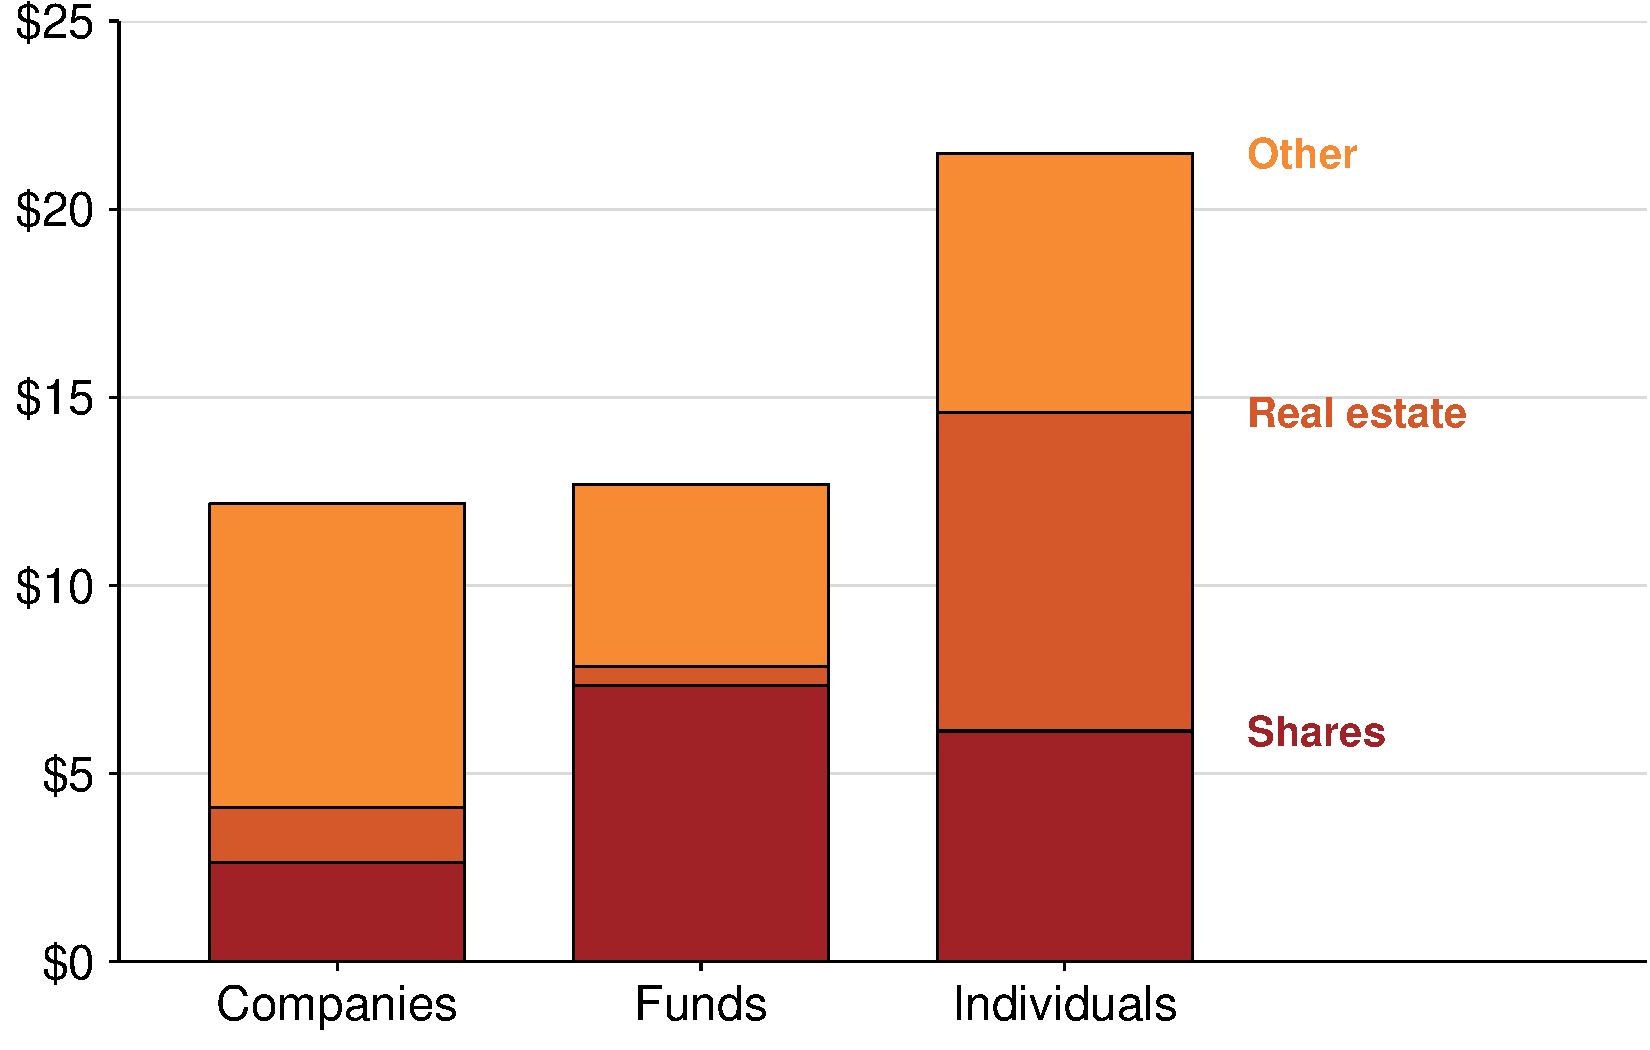
\includegraphics[width=\columnwidth]{figure/Majority_of_taxable_gains_are_earned_by_individuals-1}
\source{Molten combination of \textcite{ATOCapitalGainsByType}}
\end{figure}


\begin{smallbox}{A short history of capital gains tax changes}{box:short_history_CGT}
Before 1985 capital gains were untaxed in Australia. Taxes on capital gains were introduced to improve the integrity of the tax system, which was undermined by taxpayers recharacterising regular income as capital to avoid tax.\footcites{Evans2005}{Kenny2005}

Between 1985 and 1999, real capital gains (sale proceeds minus the original purchase price adjusted for inflation) were taxed at a taxpayer's marginal income tax rate. 

As recommended by the Ralph Review of Business Taxation, the Howard Government removed indexation adjustments so that tax was applied on nominal gains. To offset the removal of the indexation concession, capital gains tax was discounted by 50 per cent for individuals and 33 per cent for superannuation funds for assets held for more than a year. Capital gains of small unincorporated businesses, but not large businesses, are also discounted by 50 per cent. Small businesses also receive a range of other CGT concessions. When this regime was introduced, it was argued that it would stimulate capital markets and make the Australian regime more internationally competitive.\footcite[p.~14, 598]{BusinessTaxation1999} 

The tax concession is a crude way to adjust for the effects of inflation. It results in a lower tax bill compared to taxing real gains so long as asset values grow at least twice the rate of inflation. Given the strong real growth in asset prices, particularly residential property, since the discount was introduced governments have almost certainly lost revenue from the change.

\end{smallbox}
Before 1985, capital gains were not taxed in Australia. Since then, the tax treatment of capital gains has varied, but they are taxed at a lower rate than wage and salary income (\Vref{box:short_history_CGT}).  

Under the current rules, net capital gains are included as part of assessable income.\footnote{Capital losses can only be offset against capital gains, not ordinary income. But if taxpayers are unable to utilise their capital losses is a particular year, they are carried forward to future years \textcite{ATO2014a}.}  For individuals and small businesses, 50 per cent of their capital gains are excluded from income if they hold the asset for more than one year. This means the effective tax rate paid on these gains is half the rate for other forms of income. For superannuation funds, a third of their gains are excluded. Large corporations pay tax on all of their capital gains at the corporate tax rate of 30 per cent.

Capital gains have other less explicit tax advantages compared to recurrent income. Investors control when they realise gains. Consequently, they can reduce their tax by selling assets when their income is low, such as after retirement, so they are taxed at a lower marginal rate.\footnote{A common strategy for investors close to retirement is to shift capital assets into Self Managed Super Funds, and then sell them when they are aged over 60 and not liable for tax.}  For example, \textcite{Wood2010a} found that after adjusting for other factors, the probability of a landlord selling a property increases by over 20 percentage points once they retire.\footnote{The Age Pension asset test also encourages those moving into retirement to sell their assets. \textcite{Wood2010a}.}
Further, unlike other forms of income, capital gains are taxed on sale rather than as they accrue. This deferral of tax is akin to the government providing the investor with an interest free loan. (See \Vref{sec:ShouldCapitalGainsBeTaxedConsistently})

\section{Should capital gains be taxed consistently with other forms of income?}\label{sec:ShouldCapitalGainsBeTaxedConsistently}
Capital gains and other forms of savings income increase a person's spending power. It is arguable that all increases in spending power should be taxed consistently regardless of how they are earned (chapter 2)  or as the Canadian Carter report puts it ``a buck is a buck is a buck.''  But in practice, many forms of income from investments -- including owner occupied homes,  superannuation  and capital gains -- are taxed less than income from working. 

Taxing capital gains consistently with other forms of income would reduce the incentive for speculative investments and revenue leakage from artificially structured transactions. It is also highly progressive because most capital gains income is earned by the wealthy. 

On the other hand, capital gains are not the same as other forms of income. There is genuine concern that increasing taxes on capital gains might reduce incentives to save and start new businesses. But personal income tax rates are not the most important determinants of these decisions. While capital gains are eroded by inflation, so are all forms of investment returns. This does not provide a rationale for special treatment of gains. 

The most compelling reason for taxing capital gains at a lower rate is to moderate the effect of `asset lock in', whereby investors are deterred from selling assets that have accrued large gains. This could be more directly dealt with through moving to a system where gains are taxed on an accrual basis.  








\begin{figure}
\Caption{Negative gearing benefits mostly benefits those on high incomes, and the difference is especially stark when incomes are measured before subtracting rental interest deductions}{Percentage of each decile's share of the benefit in reduced income tax due to negative gearing (2012-13)}  {fig:Effect_of_Deductions}
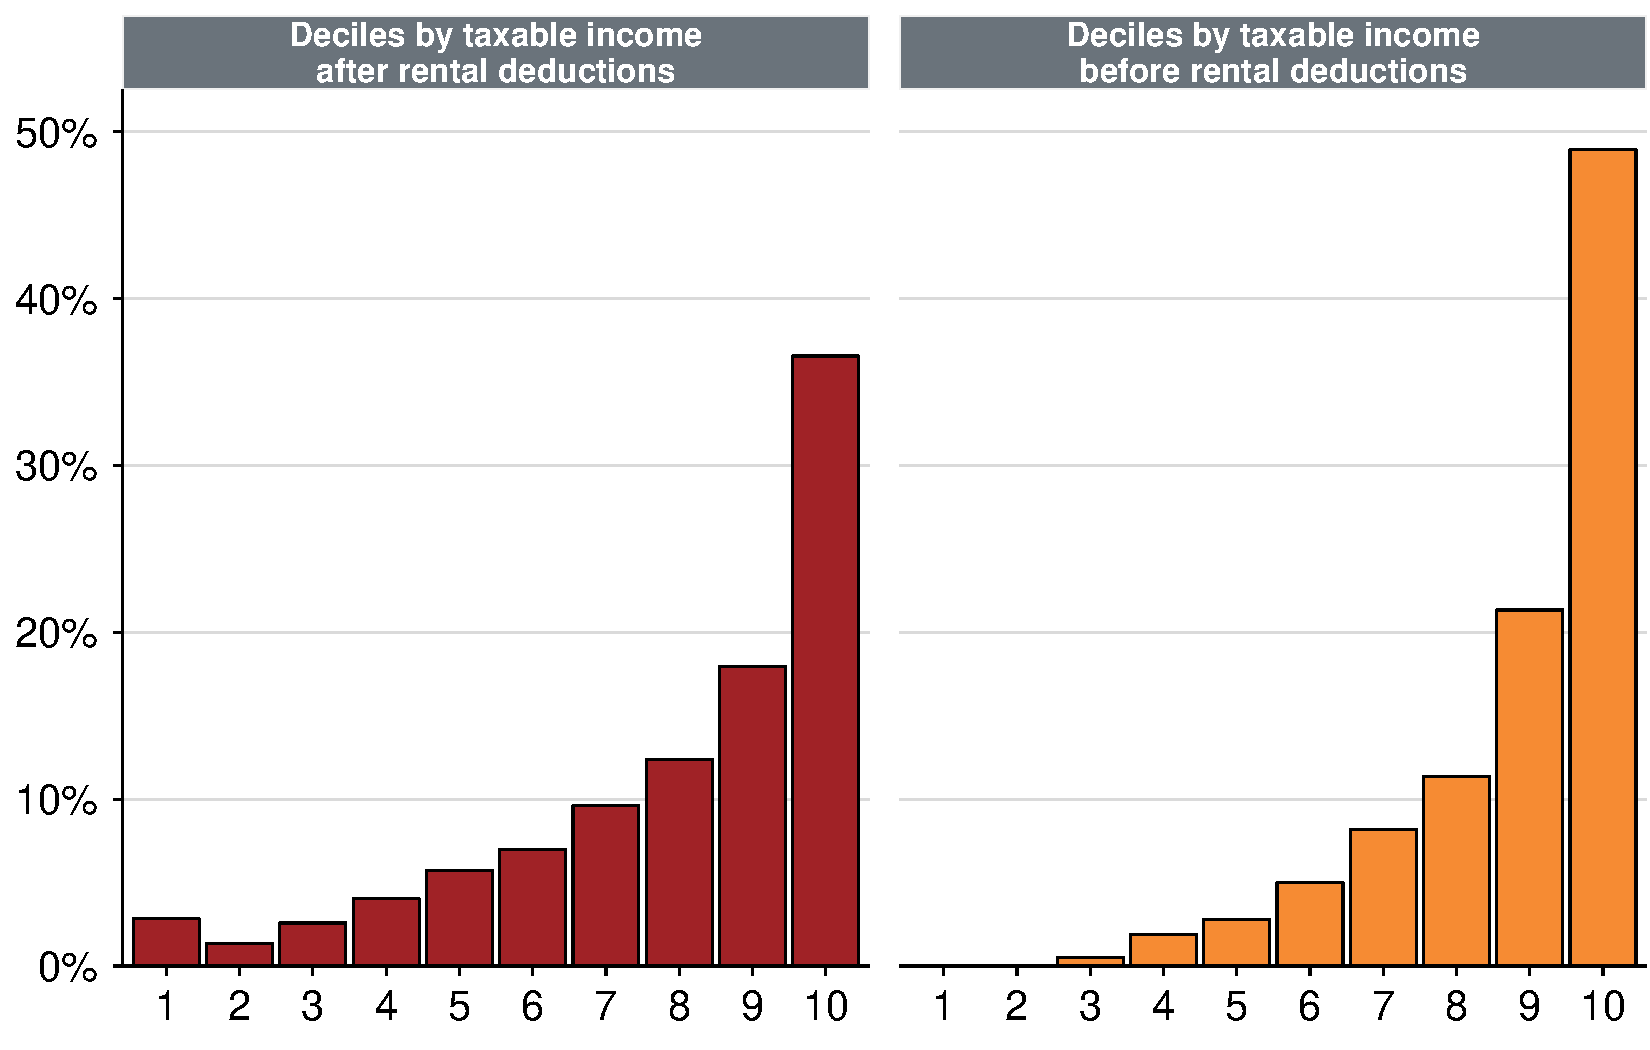
\includegraphics[width=\columnwidth]{figure/Effect_of_Deductions-1}
\notes{Income tax before rental deductions means $\text{Taxable Income} - \min(\text{Net rental profit}, 0)$. Income tax includes medicare levy, medicare thresholds, but not other tax benefits (\emph{e.g.}~the seniors and pensioners tax offset (SAPTO))}

\source{\gao \textcite{ATO2013i}}
\end{figure}


\begin{figure}
\Caption{Negative gearing benefits mostly benefits those on high incomes, and the difference is especially stark when incomes are measured before subtracting rental interest deductions}{Average amount by which income tax was reduced due to negative gearing (2012-13)}  {fig:Effect_of_Deductions_amount}
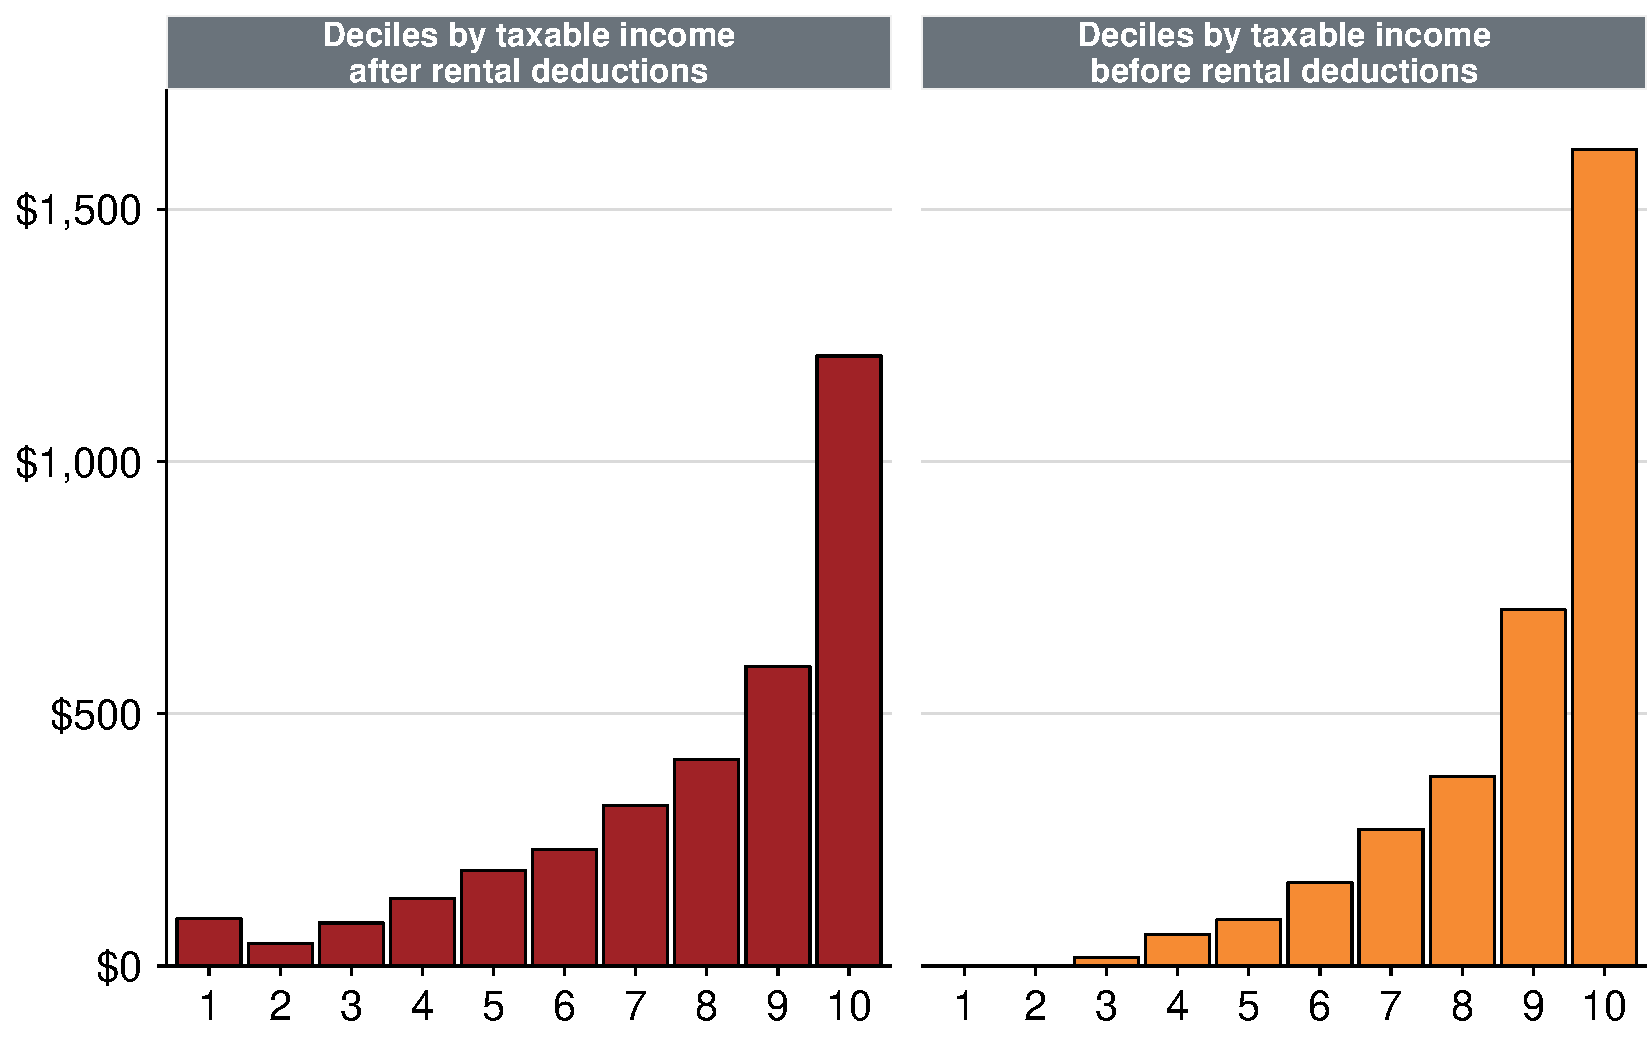
\includegraphics[width=\columnwidth]{figure/Effect_of_Deductions_amount-1}
\notes{Income tax includes medicare levy,  medicare thresholds, but not other tax benefits (\emph{e.g.}~the seniors and pensioners tax offset (SAPTO))}

\source{\gao\ \textcite{ATO2013i}}
\end{figure}
\clearpage





\begin{figure}
\Caption{}{Number of taxpayers by taxable income decile who negatively gear}{fig:NegGearing_share_by_deciles}
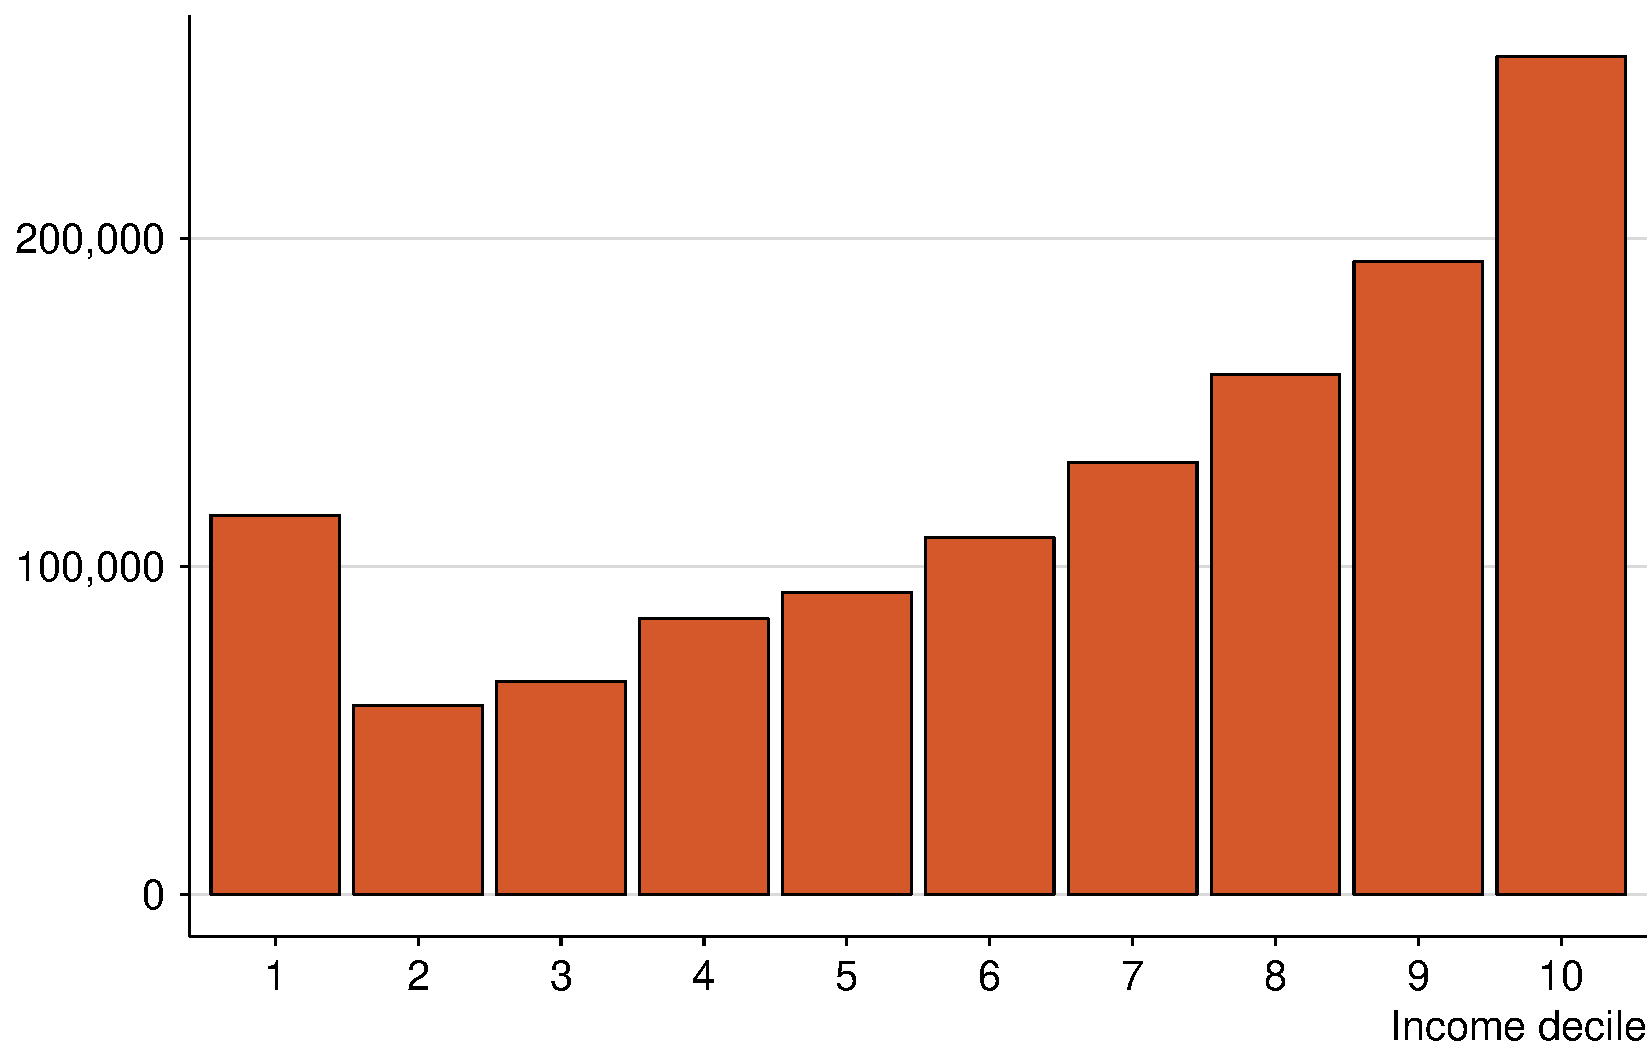
\includegraphics[width=\columnwidth]{figure/NegGearing_share_by_deciles-1}
\notes{}

\source{}
\end{figure}



\begin{figure}
\Caption{}{Total net rental losses by taxable income decile}{fig:NegGearing_amount_by_deciles}
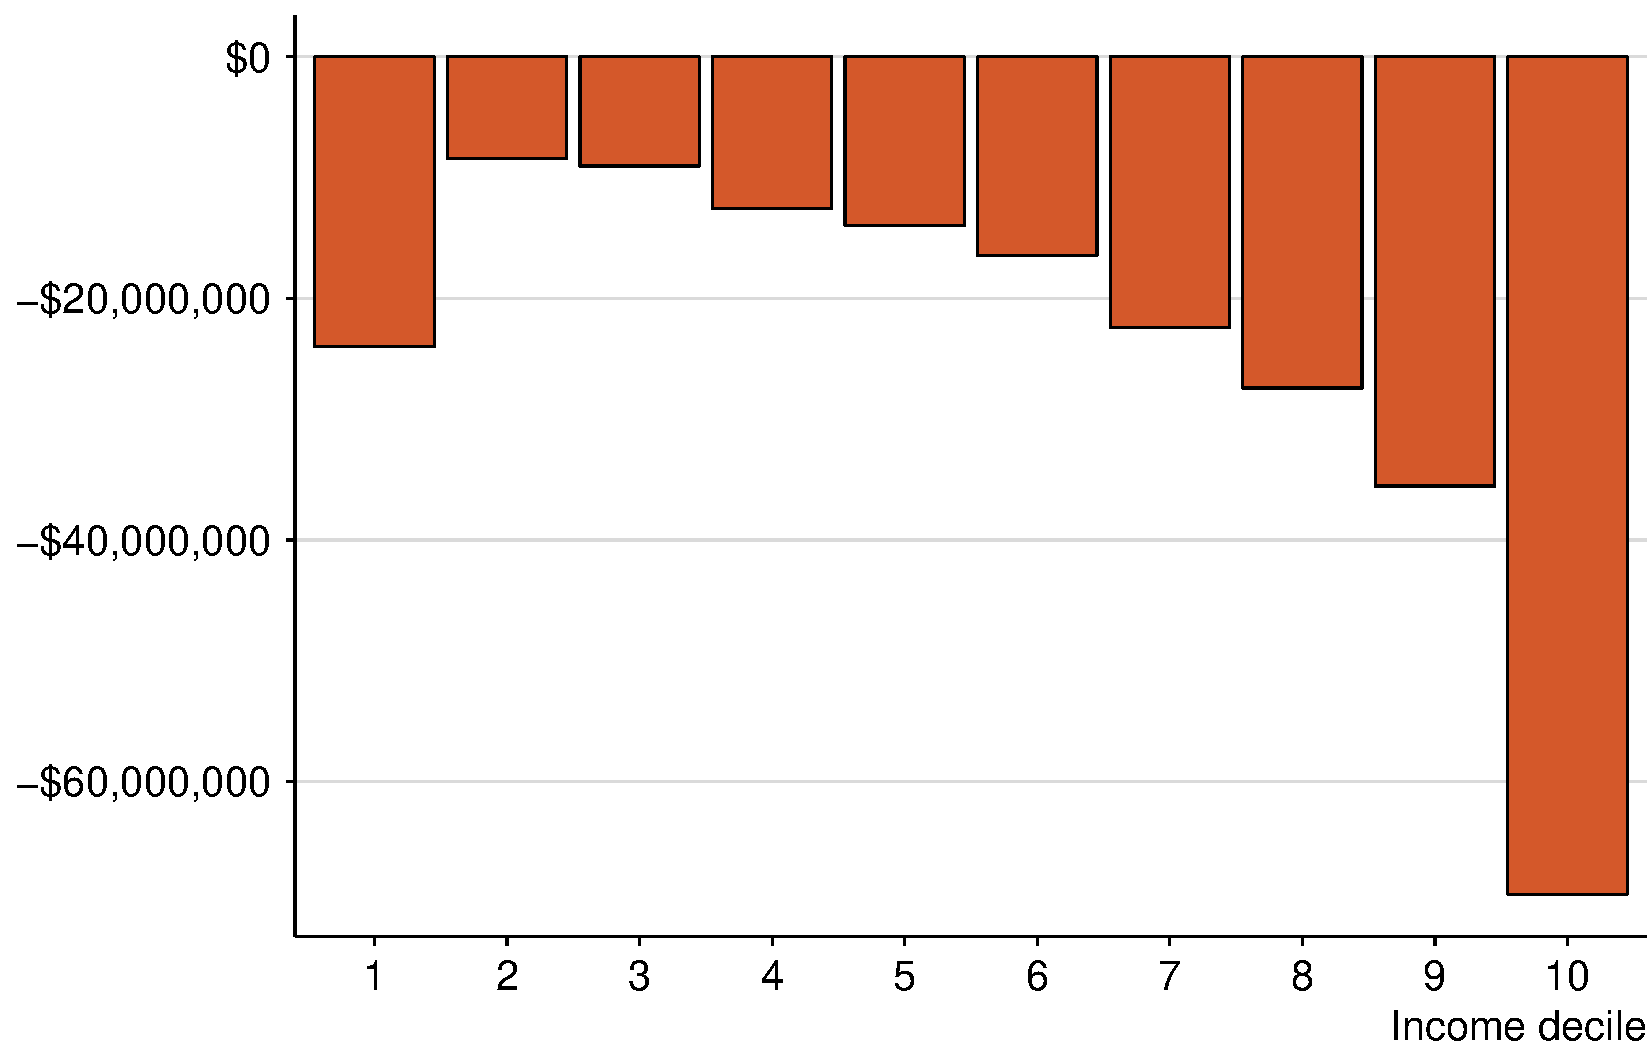
\includegraphics[width=\columnwidth]{figure/NegGearing_amount_by_deciles-1}
\notes{}

\source{}
\end{figure}



\begin{figure}
\Caption{}{Average rental losses (for those with negative net rental amounts)}{fig:NegGearing_avg_amount_by_deciles}
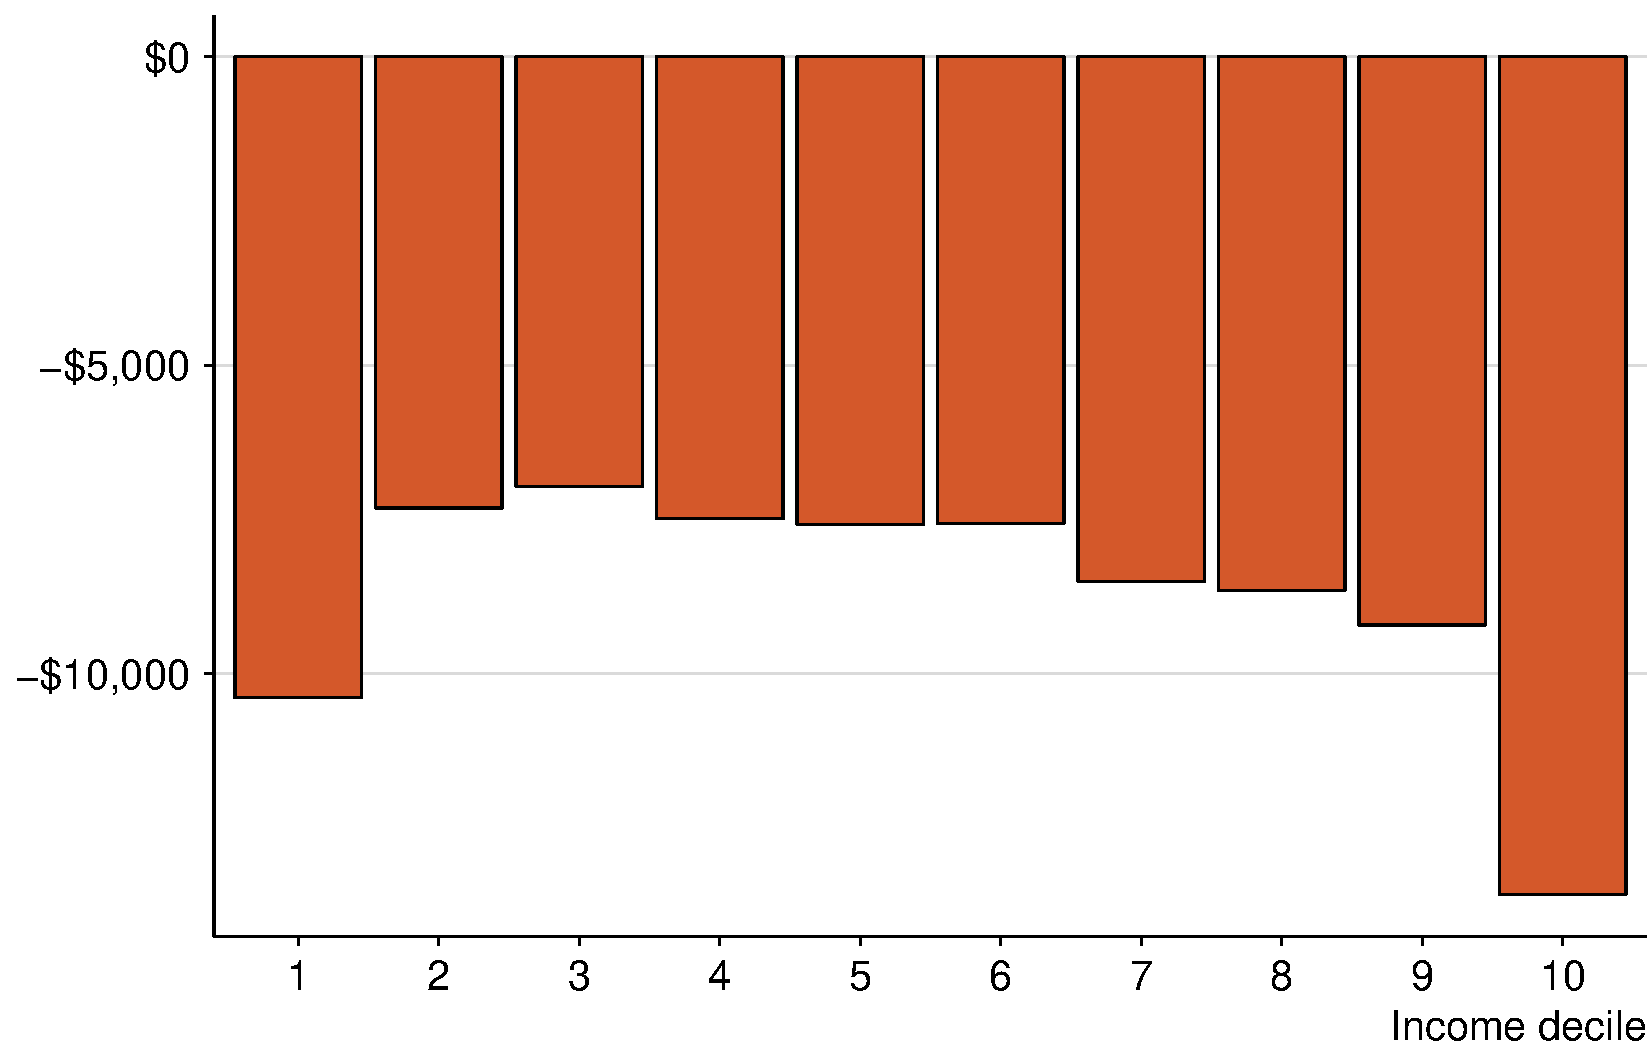
\includegraphics[width=\columnwidth]{figure/NegGearing_avg_amount_by_deciles-1}
\notes{}

\source{}
\end{figure}



\begin{figure}
\Caption{A higher proportion of taxpayers from the top income tax brackets change brackets as a consequence of negative gearing}{Number and proportion of taxpayers in each tax bracket (income determined before rental deductions) who change brackets as a result of negative gearing}{fig:Tax_brackets}
\includegraphics[width=\columnwidth]{figure2/Tax_brackets-1}
\notes{}

\source{\gao \textcite{ATO2013i}}
\end{figure}

\begin{figure}
\Caption{Negative gearing results in over 200,000 taxpayers moving down at least one tax bracket}{Number of taxpayers moving down tax brackets as a result of rental deductions}{fig:BracketFall}
 \begin{tikzpicture}[node distance = 3cm, auto]
 \tikzstyle{every node}=[font=\small]
  \node [block, fill=Color1] (Under) {0-18,200};
  \node [block, fill=Color2, above right of = Under] (Low) {18,201-37,000};
  \node [block, fill=Color3, above right of = Low] (Middle) {37,001-80,000};
  \node [block, fill=Color4, above right of = Middle] (Upper) {80,001-180,000};
  \node [block, fill=Color5, above right of = Upper] (High) {180,000+};
  %
  \path [line] (Low) --node{41,800} (Under);
  %
  \path [line] (Middle) to[out = 180, in = 90, anchor=west, fill=white]node{8450} (Under);
  \path [line] (Middle) --node{66,650} (Low);
  %
  \path [line] (Upper) --node{84,300} (Middle);
  \path [line] (Upper) to[out = 180, in = 90, anchor=south east]node{1400} (Under);
  \path [line] (Upper) to[out = -90, in = 0] node{1400} (Low);
  %
  \path [line] (High) --node[anchor=south east]{17,650} (Upper);
  \path [line] (High) to[out = 180, in = 90, anchor=south east]node{200} (Middle);
  \path [line] (High) to[out = -90, in = 0]node{100} (Under);
 \end{tikzpicture}
\end{figure}


% latex table generated in R 3.2.0 by xtable 1.7-4 package
% Sat Jun 06 21:09:03 2015
\begin{table}[ht]
\centering
\begin{tabular}{lr}
  \hline
Age & Number negatively gearing \\ 
  \hline
under 20 & 200 \\ 
  20 to 24 & 17,600 \\ 
  25 to 29 & 94,350 \\ 
  30 to 34 & 150,500 \\ 
  35 to 39 & 163,950 \\ 
  40 to 44 & 182,300 \\ 
  45 to 49 & 177,250 \\ 
  50 to 54 & 185,050 \\ 
  55 to 59 & 151,200 \\ 
  60 to 64 & 88,450 \\ 
  65 to 69 & 34,550 \\ 
  70 and over & 15,900 \\ 
   \hline
\end{tabular}
\end{table}



\begin{figure}
\Caption{The incidence of negative gearing is roughly constant for middle-aged Australians. Between 12.9\%\ and 14.8\%\ of each age group from 35 to 59 experience a net rental loss}{Percentage of taxpayers with a net rental loss, by age group}{fig:Percentage_of_taxpayers_with_a_net_rental_loss_by_age_group}
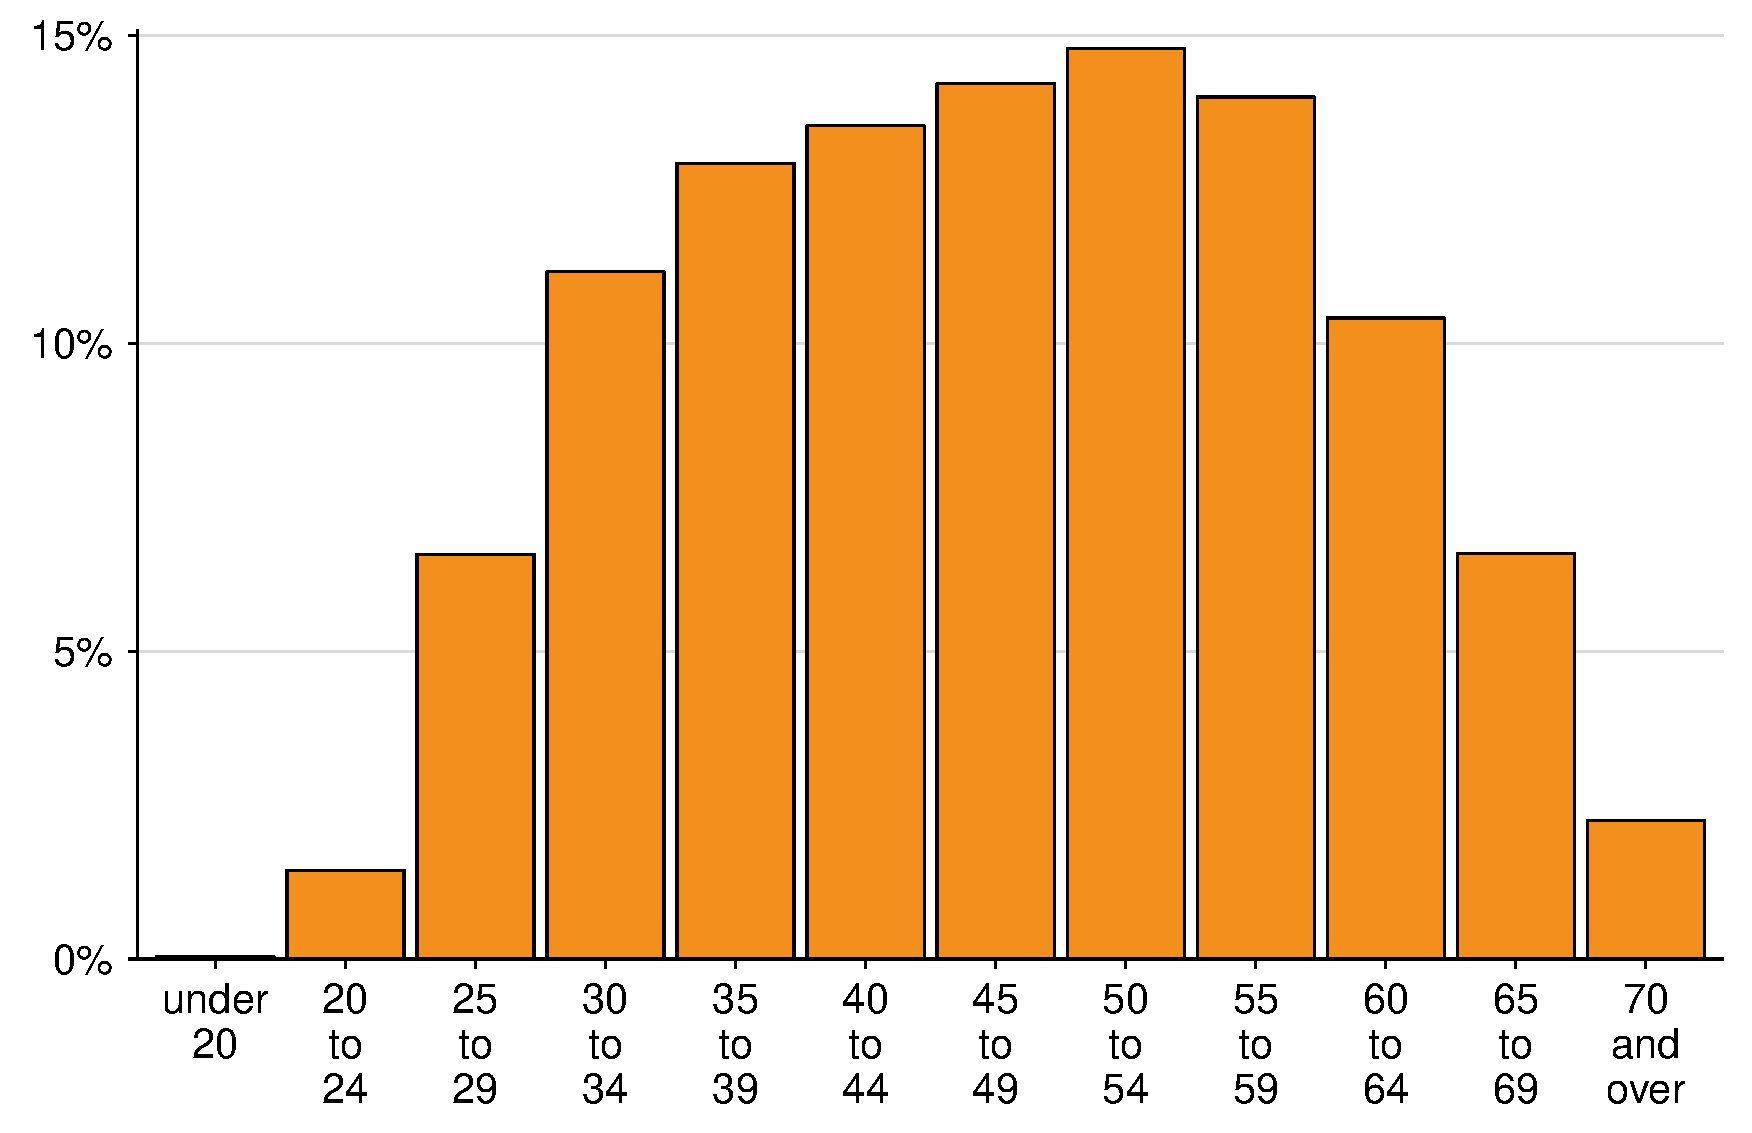
\includegraphics[width=\columnwidth]{figure/Percentage_of_taxpayers_with_a_net_rental_loss_by_age_group-1}
\notes{}

\source{\gao \textcite{ATO2013i}}
\end{figure}



\begin{figure}
\Caption{}{Number of taxpayers by type}{fig:Age_negative_gearing_not_negative_gearing}
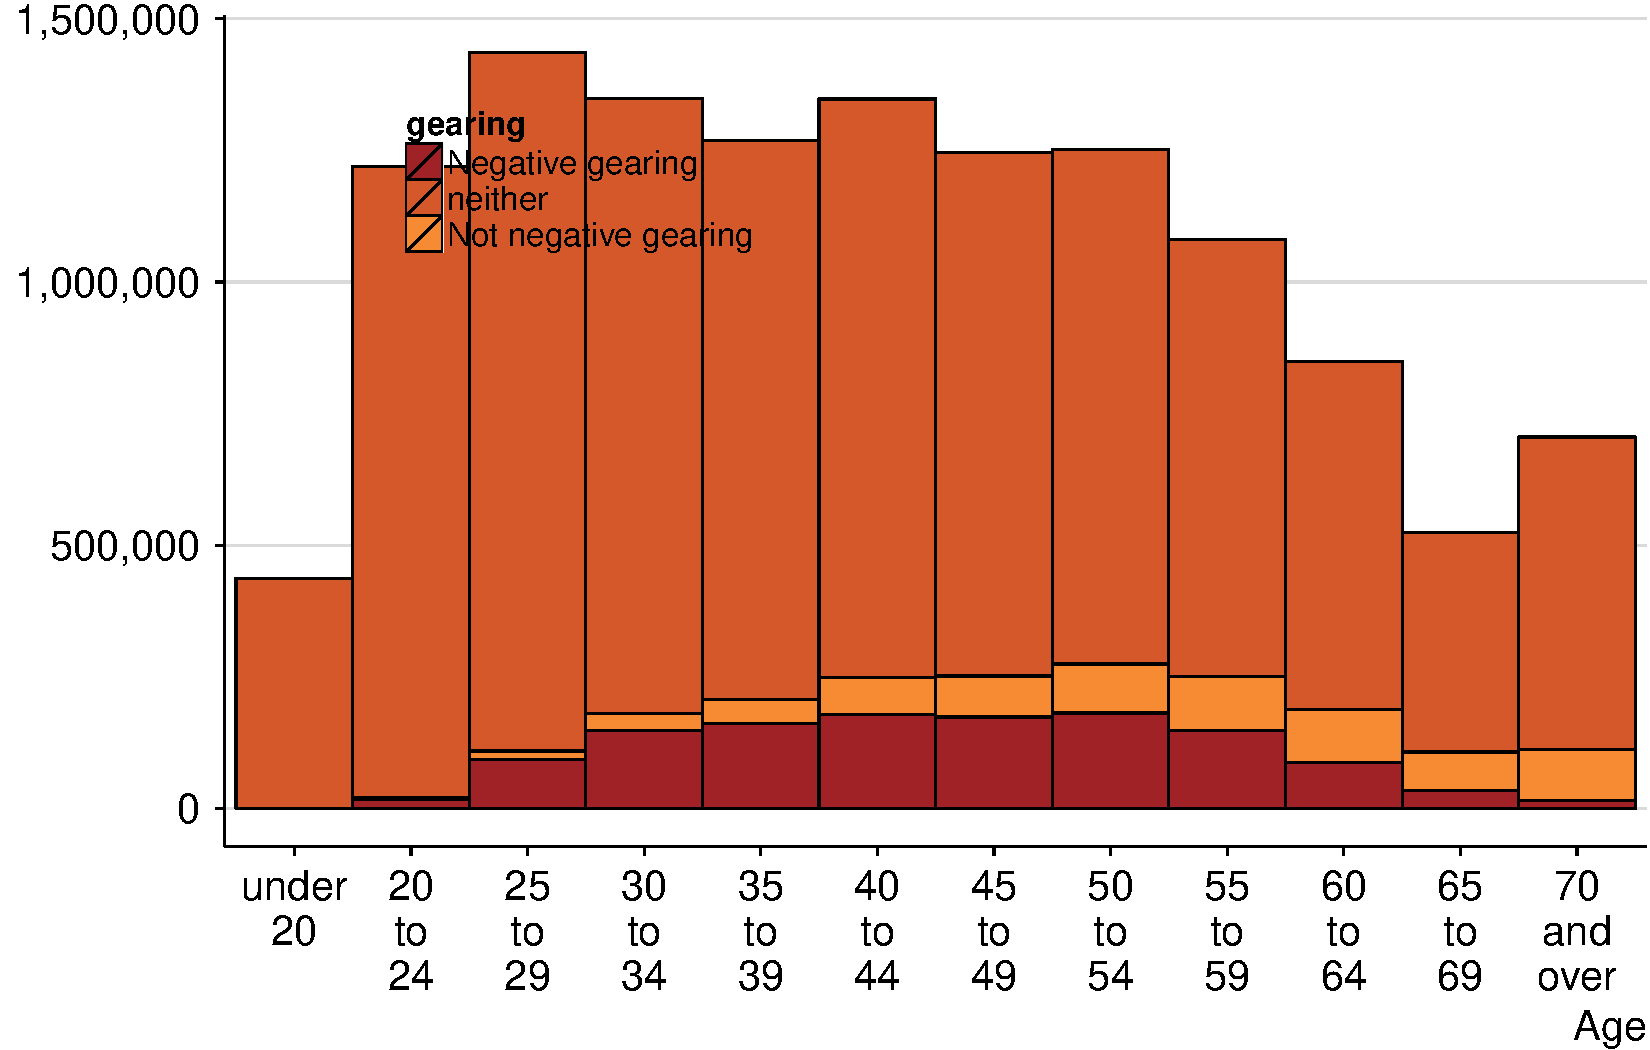
\includegraphics[width=\columnwidth]{figure/Age_negative_gearing_not_negative_gearing-1}
% \source{~\verb!Age_negative_gearing_not_negative_gearing!}
\end{figure}



\begin{figure}
\Caption{Most people with investment properties use negative gearing}{Percentage of each age group with positive rental income with net rental losses}{fig:Negatively_geared_investors_as_a_share_of_all_property_investors_by_age}
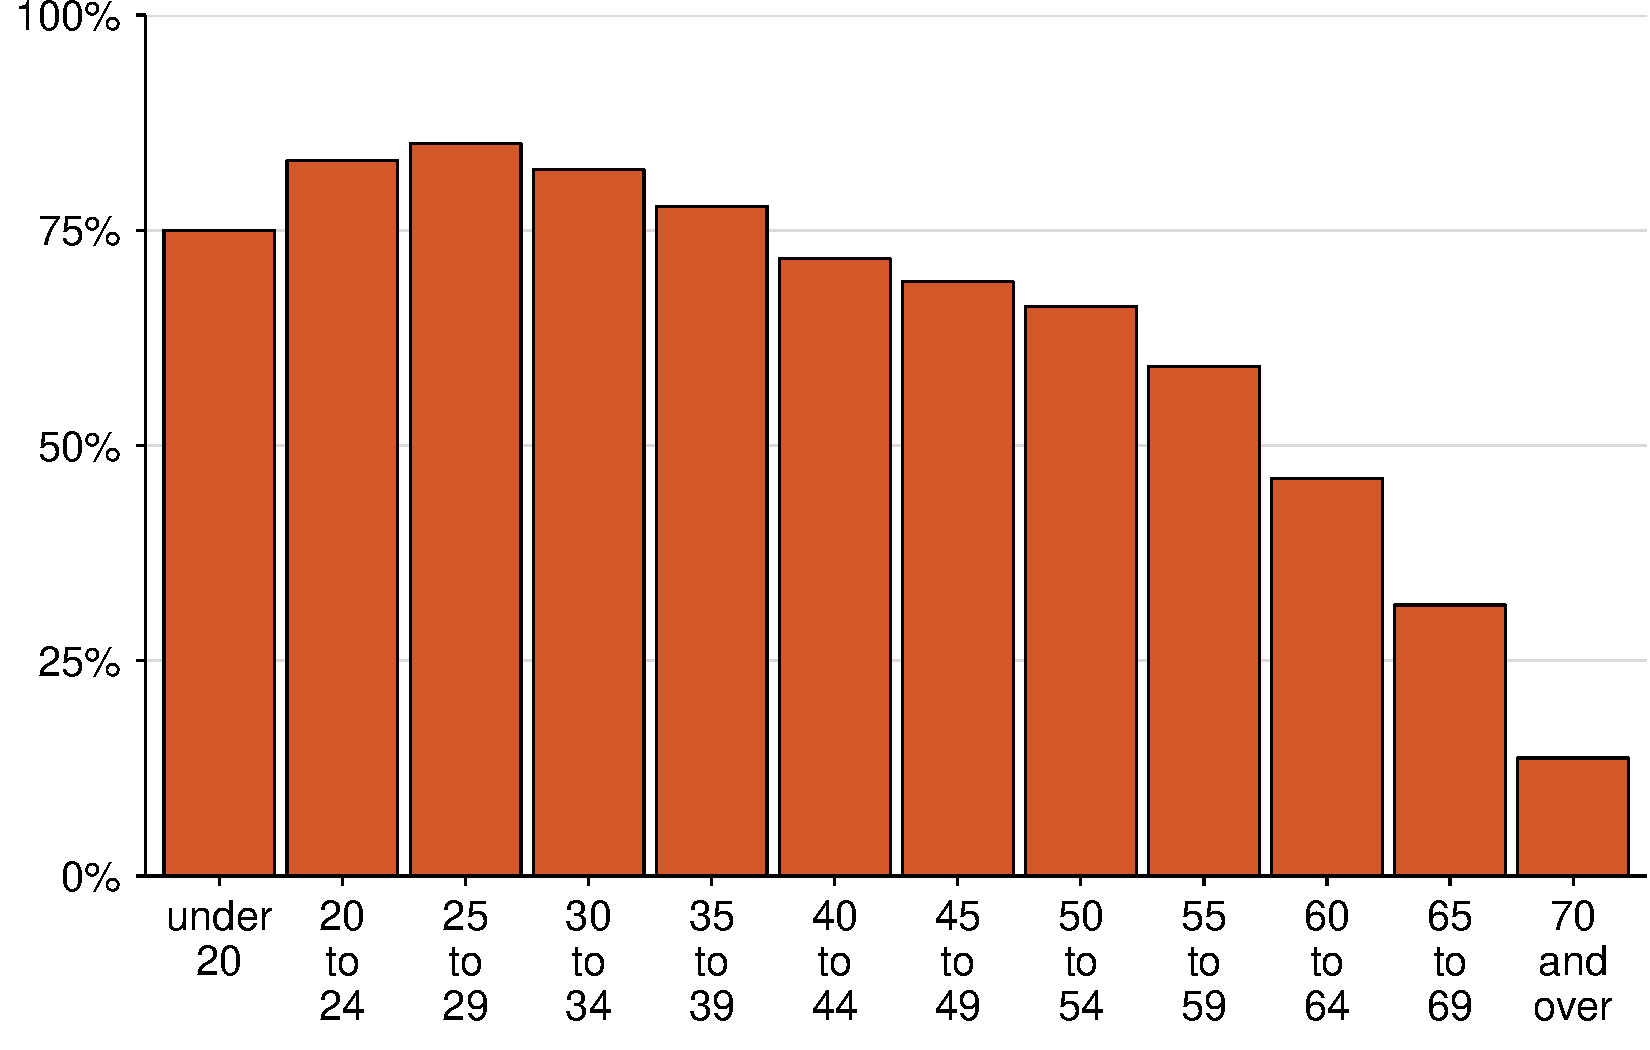
\includegraphics[width=\columnwidth]{figure/Negatively_geared_investors_as_a_share_of_all_property_investors_by_age-1}
\notes{Under 20 age group based on merely four entries in the sample file; only a tiny number of under 20s have investment properties.}

\source{\gao\textcite{ATO2013i}}
\end{figure}

\section{Capital gains distribution}
% Capital gains by income decile.

\begin{figure}
\Caption{Over two-thirds of capital gains are earned by the top 10\%\ of taxpayers}{Average net capital gains by income decile (2012-13)}{fig:Capital_gains_by_income_decile}
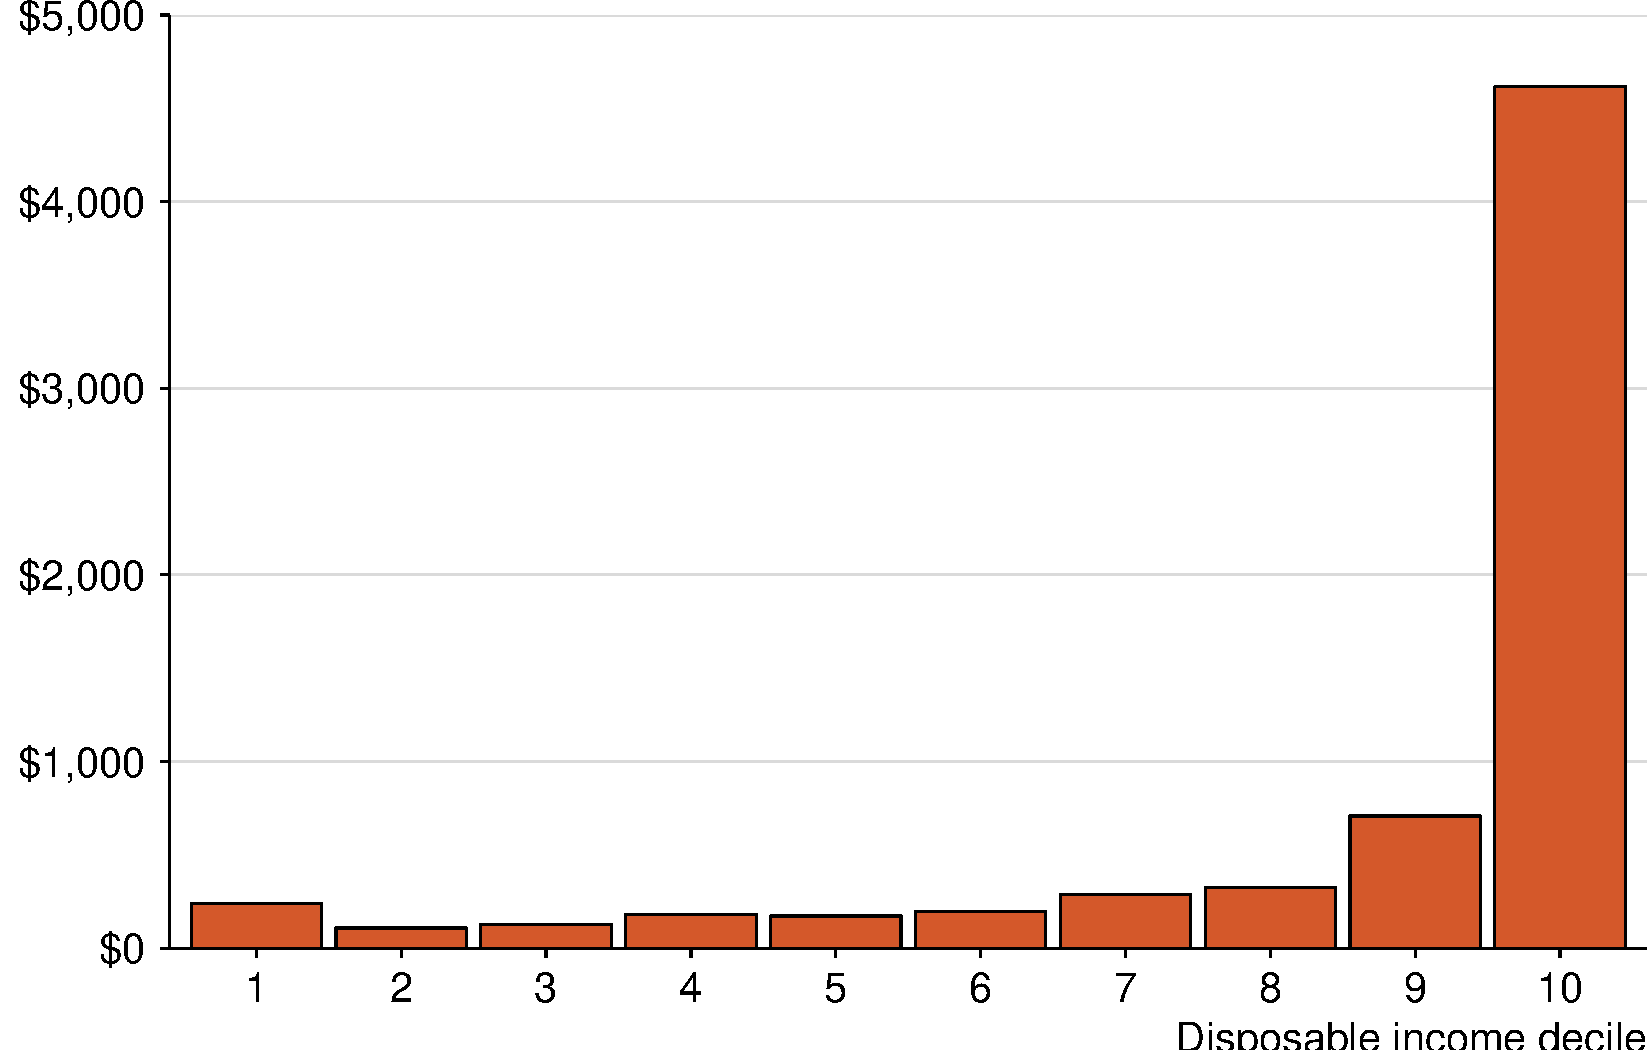
\includegraphics[width=\columnwidth]{figure/Capital_gains_by_income_decile-1}
\notes{Income based on total income reported}

\source{\gao\ \textcite{ATO2013i}}
\end{figure}
\chapter{Costings}
\section{30\%\ CGT discount and negative gearing only for the non-salary component of taxable income}
Instead of a 50\%\ discount on the amount of capital gains that may be taxed, we propose a 30\%\ discount on the component of capital gains forming one's assessable income. Further, we propose that individuals be no longer permitted to deduct losses arising from their investments against any income other than investments and capital gains; in particular, negative gearing against salaries and wages will cease.
\subsection{Status quo}
Currently, assessable income ($I_A$) is encoded directly into tax stats
\[I_A = \verb=Taxable_Income=\]
An individual's capital gains amount is recorded in Income item 18 labels A (Net capital gains) and H (Total capital gains). Item A includes the 50\%\ discount and capital losses, but item H does not.\footnote{See \url{https://www.ato.gov.au/Individuals/Tax-Return/2013/Supplementary-tax-return/Income-questions-13-24/18---Capital-gains/}} This corresponds to items \verb=Net_CG_amt= and \verb=Tot_CY_CG_amt= respectively. We thus ignore \verb=Tot_CY_CG_amt=.

Capital gains tax for individuals is not a separate tax; it is simply a component of an individual's income tax. Once the appropriate deductions and discounts have been made, it is simply added on to a person's assessable income:
\[I_A = \text{Capital gains (after discounts, deductions)} + \text{Other income}\]
and
\[\text{tax payable} = T(I_A)\]
where $T$ is not a function of capital gains, $\frac{\partial T(\cdot)}{\partial \text{Capital gain}} = 0$.
%
\subsection{Our proposal}
We need to determine:
\begin{enumerate}
\item Total capital gains (pre-discount) for each taxpayer
\item The amount they could deduct, but can no longer
\end{enumerate}
\subsubsection{Total capital gains}
Determining total capital gains from tax stats suffers from a flaw. Only the \emph{Total capital gains} $K_T$ and the \emph{Net capital gains} $K_n$ are recorded. Net capital gains is the component of an individual's income upon which the marginal tax rate is applied -- it includes both capital losses and the capital gains discount. Total capital gains is the sum of all capital gains for the year, without capital losses or the capital gains discount.

It follows that our best estimate of the total capital gains to which the discount would apply is double the \emph{Net capital gains} amount. So the assessable income under a new regime ($I_A'$) with a discount on capital gains of $d$ will be 

\[I_A' = I_A - K_n + 2K_n(1 - d).\]

\begin{smallbox}{Tax stats}{box:TaxStatsCapitalGains}
John purchases and sells (13 months later) two houses, making capital gains of \$10,000 and \$25,000. He also experienced a capital loss of $-$\$5,000 last year which has not yet been applied against later year capital gains. His total capital gains is \$35,000 and his net capital gains is \$15,000.

In our calculations, we only see that John had a total capital gain of \$35,000 and a net capital gain of \$15,000. We infer that his total capital gains was $2\times \$15,000 = \$30,000$. 
\end{smallbox}






\subsection{Negative gearing}


\subsection{Isolate salary}
Current:
\begin{align*}
I_A &= \text{Salary} + \text{Other income} \\
&\qquad{} - \text{deductions excl. rental losses} - \text{rental losses}
\end{align*}
Let:
\begin{align*}
I_S &= \text{Salary}\\
I_{A\backslash S} &= \text{Other income} \\
&\qquad{} - \text{deductions excl. rental losses} - \text{rental losses} \\
 &= I_A - I_S
\end{align*}
Then a person's assesable income under the new scenario, $I_A'$ is the person's salary where deductions are only permitted against the person's non-salary income. Deductions in excess of a person's non-salary income may not be further deducted against his salary:
\begin{align*}
I_A' &= I_S + \max\left(0, I_A - I_S \right)
\end{align*}
Note under this scenario, anyone who has a nonnegative salary \EMPH{cannot obtain a taxable loss}. Any costings using this scenario will overestimate the revenue colllectable under a scenario that violates this assumption.

\subsection{Application to taxstats}
% latex table generated in R 3.2.0 by xtable 1.7-4 package
% Sat Jun 06 21:09:11 2015
\begin{table*}[ht]
\centering
\caption{Summary table for taxable income based on $I_A' = I_S + \max(0, I_A - I_s)$.} 
\begin{tabular}{lllll}
  \hline
Net rental profit &     $I_A$ &     $I_A'$ & Tax (status quo) &   Tax (new) \\ 
  \hline
Min.   :-474901.0   & Min.   :       0   & Min.   :       0   & Min.   :      0   & Min.   :      0   \\ 
  1st Qu.:      0.0   & 1st Qu.:   21785   & 1st Qu.:   22464   & 1st Qu.:    361   & 1st Qu.:    557   \\ 
  Median :      0.0   & Median :   41561   & Median :   43178   & Median :   5301   & Median :   5875   \\ 
  Mean   :   -423.9   & Mean   :   55565   & Mean   :   57447   & Mean   :  12863   & Mean   :  13529   \\ 
  3rd Qu.:      0.0   & 3rd Qu.:   69150   & 3rd Qu.:   72111   & 3rd Qu.:  15058   & 3rd Qu.:  16065   \\ 
  Max.   : 474433.0   & Max.   :12584567   & Max.   :12584567   & Max.   :6014139   & Max.   :6014139   \\ 
   \hline
\end{tabular}
\end{table*}

So under the current regime where \$163.6~billion is payable in income tax, the above scenario renders \$172~billion payable.
\clearpage


\subsection{Time series}





\section{Henry-lite proposal}
The proposal in the Henry review is to reduce both the capital gains discount and the amount one can deduct through negative gearing. In particular, the tax review proposes the discount be reduced to 40\%\ and a discount of 40\%\ be applied to both rental losses and rental income.\footnote{The income tax treatment of these household savings would be improved by applying a
40 per cent discount to most interest income, net residential rental property income, capital
gains and certain interest expenses. Doing so would provide a more consistent tax
outcome for income from bank deposits and bonds, shares, and rental properties, and
provide a means of adjusting for the effect of inflation. \textcite{Treasury2010a}.}




\begin{figure}
\Caption{Henry tax proposal would impose a modest extra burden, and only on those in the top deciles}{Average income tax under both systems}{fig:Henry_proposal_change_in_tax_burden_by_decile}
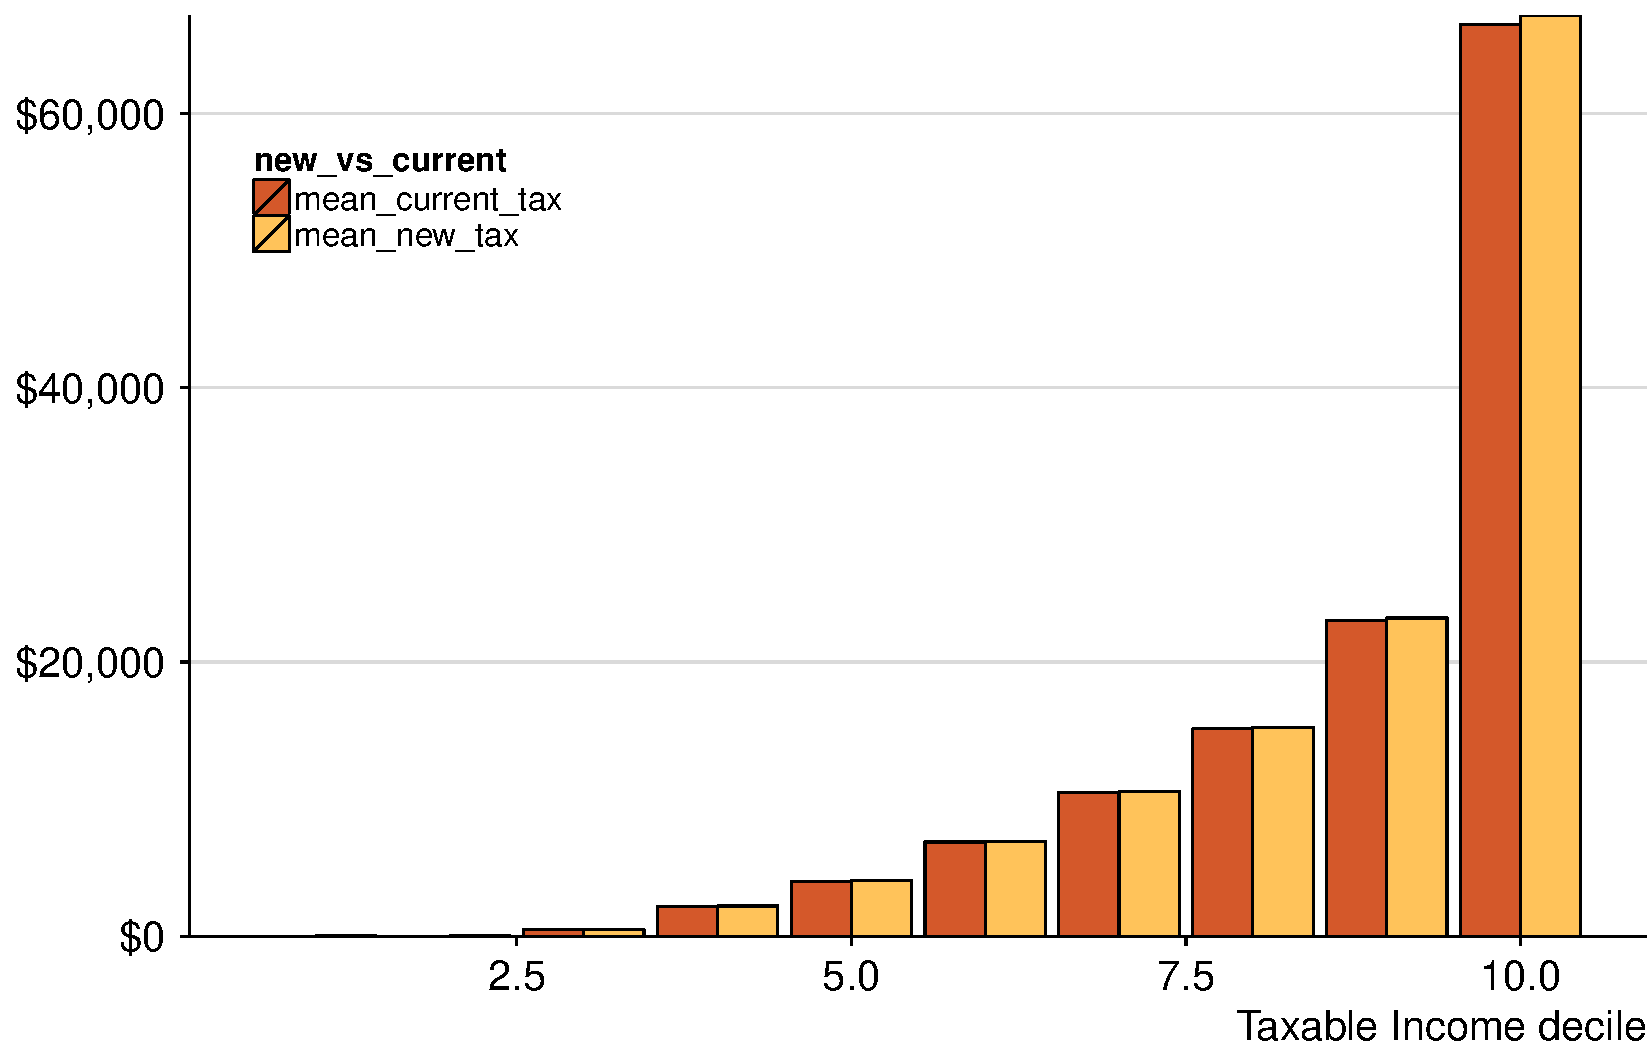
\includegraphics[width=\columnwidth]{figure/Henry_proposal_change_in_tax_burden_by_decile-1}
\notes{}

\source{}
\end{figure}

Under this proposal, income tax would rise from \$163.6~billion to \$165.1~billion.

\section{Daley (30\%\ symmetrical discount)}

Under this proposal, income tax would rise from \$163.6~billion to \$166.3~billion.







\printbibliography
\end{document}
